\documentclass{hfutpaper}
\usepackage[urlcolor=blue]{hyperref}
\usepackage{threeparttable}
\usepackage{setspace}
\usepackage{titlesec}
\usepackage{graphicx}
\graphicspath{{figures/}}
\usepackage{float}
\usepackage{cite}


\usepackage{subfigure}
\newcommand{\upcite}[1]{\textsuperscript{\textsuperscript{\cite{#1}}}}
\usepackage{fancyhdr}
% Copyright 20120 Liutao Tian, MIT License
% https://github.com/andy123t/code-latex-style/

\usepackage{listings,color}

% Matlab highlight color settings
%\definecolor{mBasic}{RGB}{248,248,242}       % default
\definecolor{mKeyword}{RGB}{0,0,255}          % bule
\definecolor{mString}{RGB}{160,32,240}        % purple
\definecolor{mComment}{RGB}{34,139,34}        % green
\definecolor{mBackground}{RGB}{245,245,245}   % lightgrey
\definecolor{mNumber}{RGB}{134,145,148}       % gray

\definecolor{Numberbg}{RGB}{237,240,241}     % lightgrey

% Python highlight color settings
%\definecolor{pBasic}{RGB}{248, 248, 242}     % default
\definecolor{pKeyword}{RGB}{228,0,128}        % magenta
\definecolor{pString}{RGB}{148,0,209}         % purple
\definecolor{pComment}{RGB}{117,113,94}       % gray
\definecolor{pIdentifier}{RGB}{166, 226, 46}  %
\definecolor{pBackground}{RGB}{245,245,245}   % lightgrey
\definecolor{pNumber}{RGB}{134,145,148}       % gray

\lstnewenvironment{Python}[1]{
	\lstset{language=python,               % choose the language of the code
		xleftmargin=30pt,
		xrightmargin=10pt,
		frame=l,
		framesep=15pt,%framerule=0pt,  % sets the frame style
		%frame=shadowbox,rulesepcolor=\color{red!20!green!20!blue!20},
		%basicstyle=\small\ttfamily,          % sets font style for the code
		basicstyle=\footnotesize\fontspec{Consolas},
		keywordstyle=\color{pKeyword},       % sets color for keywords
		stringstyle=\color{pString},         % sets color for strings
		commentstyle=\color{pComment},       % sets color for comments
		backgroundcolor=\color{pBackground}, % choose the background color
		title=#1,                            %\lstname show the filename of files
		emph={format_string,eff_ana_bf,permute,eff_ana_btr},
		emphstyle=\color{pIdentifier}
		showspaces=false,                    % show spaces adding particular underscores
		showstringspaces=false,              % underline spaces within strings
		showtabs=false,                      % show tabs within strings adding particular underscores
		tabsize=4,                           % sets default tabsize to 2 spaces
		captionpos=t,                        % sets the caption-position to bottom
		breaklines=true,                     % sets automatic line breaking
		framexleftmargin=5pt,
		fillcolor=\color{Numberbg},
		rulecolor=\color{Numberbg},
		numberstyle=\tiny\color{pNumber},
		numbersep=9pt,                      % how far the line-numbers are from the code
		numbers=left,                        % where to put the line-numbers
		stepnumber=1,                        % the step between two line-numbers.
}}{}

\lstnewenvironment{Python1}[1]{
\lstset{language=python,               % choose the language of the code
  xleftmargin=30pt,
  xrightmargin=10pt,
  frame=l,
  framesep=15pt,%framerule=0pt,  % sets the frame style
  %frame=shadowbox,rulesepcolor=\color{red!20!green!20!blue!20},
  %basicstyle=\small\ttfamily,          % sets font style for the code
  basicstyle=\footnotesize\fontspec{Consolas},
  keywordstyle=\color{pKeyword},       % sets color for keywords
  stringstyle=\color{pString},         % sets color for strings
  commentstyle=\color{pComment},       % sets color for comments
  backgroundcolor=\color{pBackground}, % choose the background color
  title=#1,                            %\lstname show the filename of files
  emph={format_string,eff_ana_bf,permute,eff_ana_btr},
  emphstyle=\color{pIdentifier}
  showspaces=false,                    % show spaces adding particular underscores
  showstringspaces=false,              % underline spaces within strings
  showtabs=false,                      % show tabs within strings adding particular underscores
  tabsize=4,                           % sets default tabsize to 2 spaces
  captionpos=t,                        % sets the caption-position to bottom
  breaklines=true,                     % sets automatic line breaking
  framexleftmargin=5pt,
  fillcolor=\color{Numberbg},
  rulecolor=\color{Numberbg},
  numberstyle=\tiny\color{pNumber},
  numbersep=9pt,                      % how far the line-numbers are from the code
  numbers=left,                        % where to put the line-numbers
  stepnumber=1,                        % the step between two line-numbers.
}}{}



\titleformat{\section}{\large \heiti}{\chinese{section}、}{0em}{}
\begin{document}
	\begin{center}
		\LARGE
		\textbf{SVD在图像压缩上的应用}\\
		\vspace{0.2em}
		\large
		作者:谢唯嘉 \ 学号:6120210299 \\ 
		专业班级:信息与通信工程 信研1班
	\end{center}
	\rule[0.1\baselineskip]{\textwidth}{0.5pt}
	\textbf{摘 \ 要}\\
	\large
	在很多情况下,数据的一小部分包含了数据的绝大部分信息,用线性代数的许多矩阵分解方法都可以将矩阵特征表现成新的易于理解的形式,在这一过程之中,实际是一个提取数据集合特征值的过程(降噪),有利于我们提高算法的精准度,减少数据运算量。 最常见的矩阵分解算法就是矩阵奇异值分解(SVD),SVD 在图像压缩、推荐系统、金融数学等领域都有应用,著名的主成成分分析算法(PCA)也是通过 SVD 实现的。
	\\
	\textbf{关键词}:SVD\quad 压缩\quad 图像\\
	\rule[0.1\baselineskip]{\textwidth}{0.5pt}
	\section{引言}
	数字图像的数据量庞大,存在较强的内在相关性,所以有必要对数字图像进行压缩(编码),减少其相关性,形成高效的表示方法。图像压缩对于人们在存储空间较小的计算机中存储图像和在某个网页中更快地加载图像来说是非常必要的\cite{ranade2007variation}。随着信息通信技术和互联网发展的新发展,包括数字化和无损压缩技术在内的这一问题在不久的将来可以得到完全解决\cite{nixon2019feature}。事实上,我们在互联网上遇到的大多数图片都是经过压缩的\cite{image}。例如,jpeg、png和gif格式都是压缩的。虽然图像压缩不可避免地会导致图像质量的下降,但是一些琐碎的字符却不值得人们关注。因此,相比图像质量的一点点损失和图像存储空间的急剧减少,我们更喜欢压缩的图像。在对这个问题进行了一些研究之后,我们打算使用奇异值分解(SVD)的知识。通过选取一些较大的奇异值和相应的左右奇异向量,我们可以用较少的数据来表示退化较小的图像。
	
	\section{图像压缩的理论基础}
	\subsection{图像存储原理}
	图像其实是利用二维坐标指定的空间数据。摄像机所获得的亮度转换成信号,在经过A/D转换器处理,作为一个值存储在计算机内,可通过图像坐标x,y进行查询。由此可见计算机以矩阵的形式存储图像,而图像为一个点阵。对于RGB图像,每幅图像都匹配一个三维张量,这个张量可以看作是三个矩阵的组合。这个张量中三个矩阵的大小与原始图片大小一样。在计算机中,有三个从0到255的整数对应于图像的每个像素。这三个整数的值分别表示像素在R-通道,G -通道和B-通道中的属性。实际上,整数首先被规范化为从0到1的浮点数,每个浮点数占用计算机存储的1字节。对于一个RGB类型的图片有m$\times$n个像素点,我们需要大约3$\times$m$\times$n比特进行存储。
	\begin{figure}[H]
		\centering
		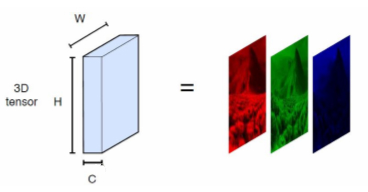
\includegraphics[scale=0.7]{1}
		\caption{图片中像素可分为RGB三通道}
	\end{figure}
	\subsection{奇异值分解的原理}
	\subsubsection{特征值和对角化}
	\textbf{特征值和特征向量}
	
	如果一个ν是方阵A的特征向量,我们可以得到以下形式:
	$$Av=\lambda v$$
	$\lambda$被称为特征值,v被称为特征向量。
	
	\textbf{对角化}
	
	如果n$\times$n方阵A有n个线性无关的特征向量,则矩阵A可以对角化,这意味着我们可以得到以下形式:
	$$P^{-1}AP=\Lambda$$
	P的列是 A的特征向量,矩阵$\Lambda$是一个对角矩阵,对角项分别是A对应于P中的特征向量的特征值。
	\subsubsection{对称矩阵与正交可对角化矩阵}
	
	如果A是对称矩阵(即A=$A^T$),它可以被正交对角化。
	$$Q^{-1}AQ=\Lambda$$
	其中Q是正交矩阵($Q^{-1}=Q^T$)。
	
	或者另一种形式:
	$$A=Q\Sigma Q^{-1}$$
	这是一种特殊的特征值分解。
	\subsubsection{奇异值分解(SVD)}
	之前介绍的特征值分解只能应用于某些方阵,这意味着它是有限的。因此,如果我们想要得到一个更一般的矩阵的分解方式(例如,一个m$\times$n矩阵,$m \neq n$)
	我们应该找另一种方法\cite{1}。
	
	我们假设矩阵A可以分解为以下形式:
	$$A=U_{m\times m}
	\begin{pmatrix}
		\sigma_{1}\\
		& \ddots & &\\
		& &\sigma_{\gamma }&\\
		& & & 0
	\end{pmatrix}_{m\times n}V^T_{n\times n}=U\Sigma V^T
	$$
	(U和V是标准正交矩阵)
	
	SVD分解的目的,如果有接近0的奇异值,可以不进行计算,一方面可以减少计算量,另一方面可以过滤噪声。
	\subsection{SVD在图像压缩上的应用}
	我们知道任何RGB模型图像都可以存储到一个具有3个通道的3D张量中。因此,我们可以压缩每个通道中的矩阵,并将它们组合在一起得到压缩图像。如前所述,任何m×n矩阵都可以分解为以下形式:
		$$A_{m\times n}=U_{m\times m}
	\begin{pmatrix}
		\sigma_{1}\\
		& \ddots & &\\
		& &\sigma_{\gamma }&\\
		& & & 0
	\end{pmatrix}_{m\times n}V^T_{n\times n}=U\Sigma V^T
	$$
	
	我们可以用谱分解的形式重写这个矩阵。奇异值可以看作是不同矩阵的权值。而奇异值越大的分解子矩阵对结果的影响越大,提供的信息也越多。因此,在进行奇异值分解时,我们倾向于将较大的奇异值重新排列在前面。因此,我们只需要选择前k个奇异值及其对应的向量,就可以代表退化程度相对较小的原始图像。假设我们有一个m$\times$n像素的图像。然后我们需要3$\times$m$\times$n比特去存储它。然而,在进行奇异值分解并选择前k个奇异值后,它只会占用3k(m+n+1)字节。事实上,k$\ll$m 和 k$\ll$n ,因此图像的存储空间大大缩小,较为直观的表现在于图像的大小成倍减少。我们设$\frac{k(m+n+1)}{m\times n}$为压缩比。

	\section{图像压缩实验}
	\subsection{代码实现}
	整体SVD在图像压缩上的应用代码基于Python语言进行编程。通过numpy函数库进行矩阵的各种运算操作,通过pillow函数库对于处理好的图像进行显现与保存。具体运行代码如下:
	\begin{Python}{图像压缩}
import numpy as np
from PIL import Image

# 使用奇异值总和的百分比进行筛选
def svd(data,scale):
# scale 代表你要保留的奇异值比例
	u,sigma,v = np.linalg.svd(data)
	svd_data = np.zeros(data.shape)
	total = sum(sigma)
	sum_data = 0
	for index,item in enumerate(sigma):  
		svd_data += item * np.dot(u[:,index].reshape(-1,1),v[index,:].reshape(1,-1))
		sum_data += item
		if sum_data >= scale * total:
			break
	return svd_data

def compress(data,scale):
#获得图片RGB三通道数并进行压缩
	r = svd(data[:,:,0],scale)
	g = svd(data[:,:,1],scale)
	b = svd(data[:,:,2],scale)
	
	result = np.stack((r,g,b),2)
	result[result > 255] = 255
	result[result < 0] = 0
	result = result.astype(int)
	return result

if __name__ == '__main__':
	image = Image.open('supercar.jpeg')
	width,height = image.size
	arr = np.zeros((width,height,3)) # RGB 
	for x in range(width):
		for y in range(height):
			arr[x][y] = image.getpixel((x, y))
	# 原生 range 不支持浮点数,所以用 np.arange 代替
	for c in np.arange(.1,1.,.2): #(.1,.9,.2)
		result = compress(arr,c)
		for x in range(width):
			for y in range(height):
				image.putpixel((x, y),(result[x,y,0],result[x,y,1],result[x,y,2]))
		image.save('test_'+str(int(100 * c))+'%.jpeg')

	\end{Python}
上述代码具体操作步骤:

\textbf{第一步:}利用PIL中的Image模块将要进行压缩的图片进行读取,并获得图片的宽和高。

\textbf{第二步:}利用PIL中的getpixel模块获取输入图像中的某一点的像素的RGB颜色值。

\textbf{第三步:}程序进入图片压缩循环,通过设置要保存的奇异值比例对图像进行压缩处理并进行保存图片。

	\subsection{实验结果与评价指标}
	\subsubsection{实验结果}
	整个实验中用图为网络用图,调用代码生成拥有不同保留比例奇异值的图片。以下为实验结果生成的图\ref{fig4}。
\begin{figure}[htbp]
	\centering
	\begin{minipage}{0.32\linewidth}	
		\centering
		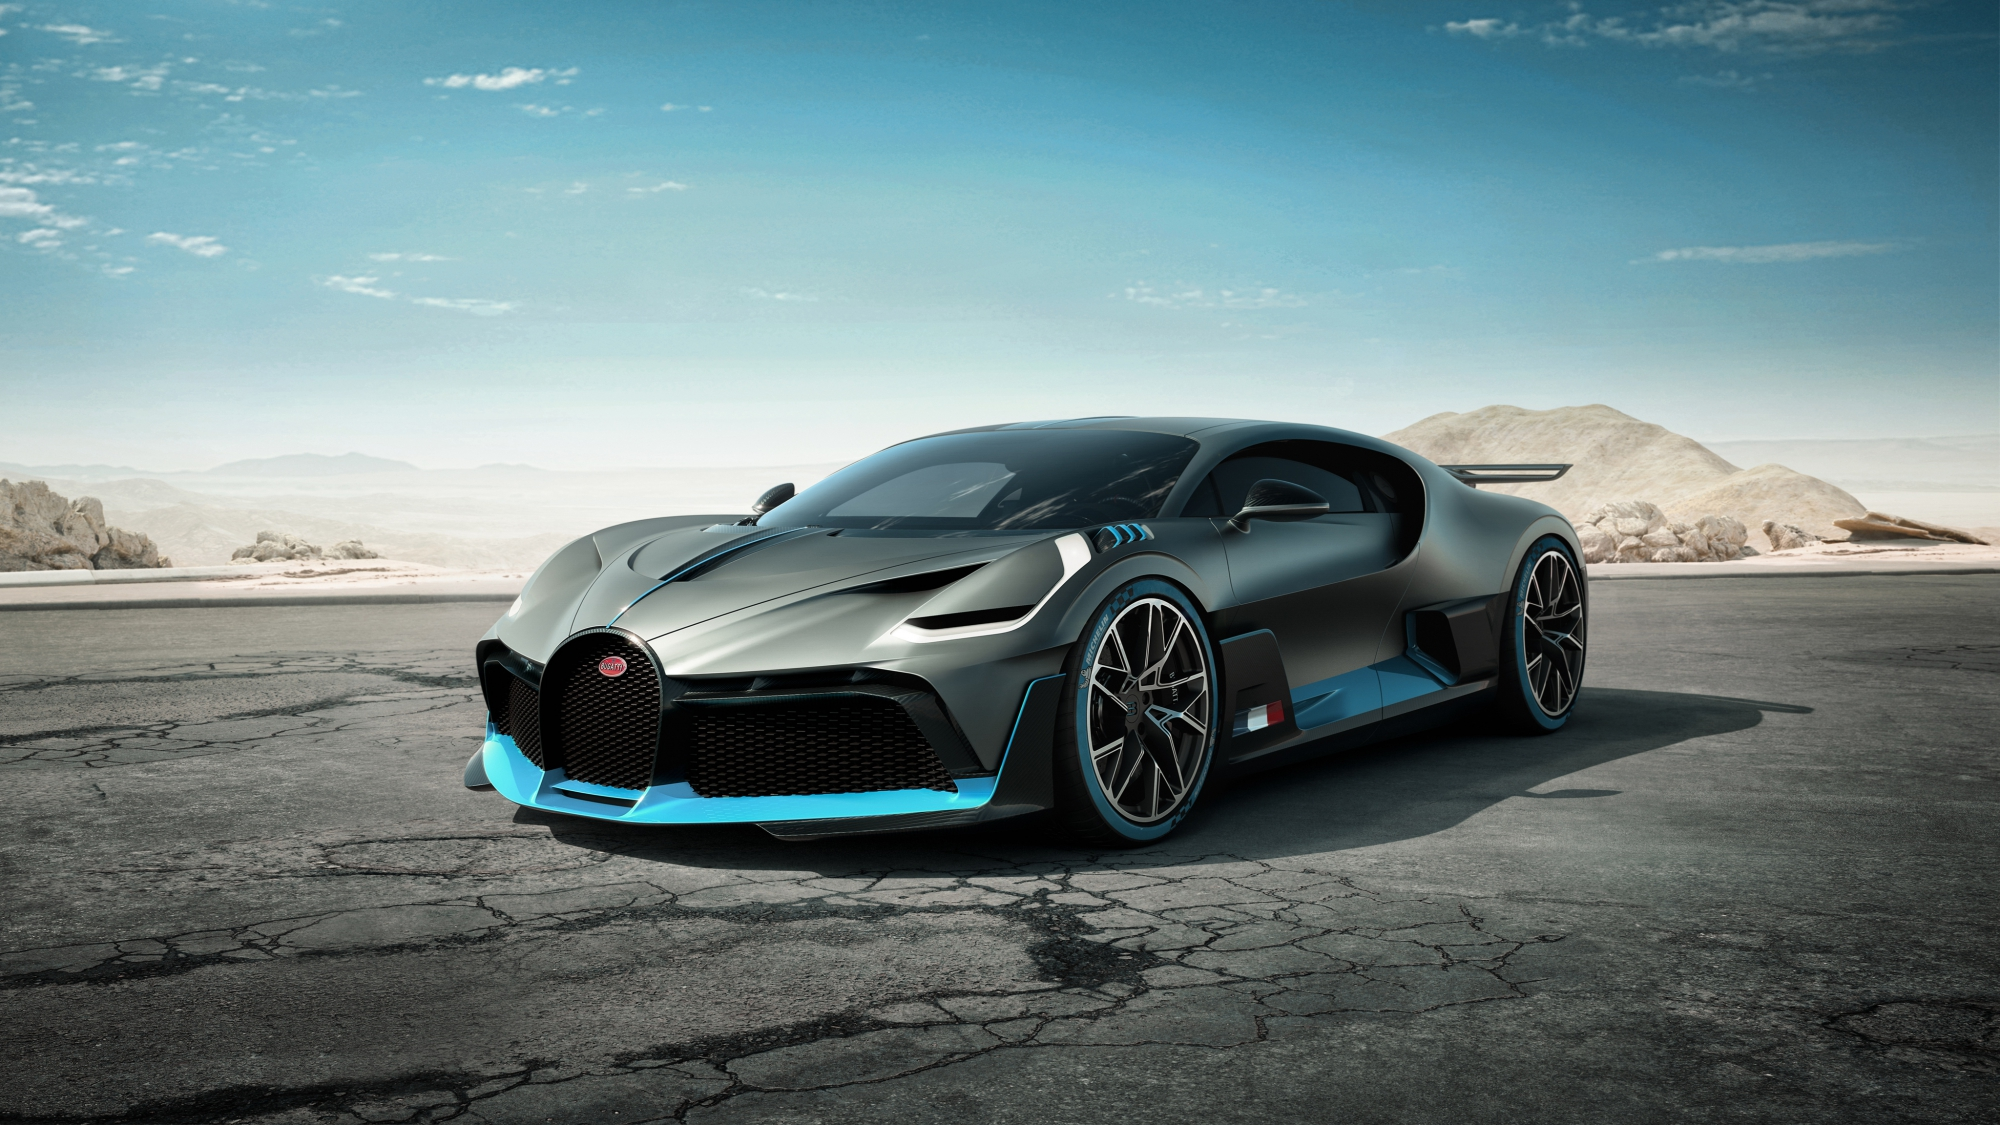
\includegraphics[width=5cm,height=3.5cm]{supercar.jpeg}
		\centerline{原始图像}	
	\end{minipage}
	\begin{minipage}{0.32\linewidth}	
		\centering
		
\includegraphics[width=5cm,height=3.5cm]{test1.jpeg}
		\centerline{保留10\%}	
	\end{minipage}
	\begin{minipage}{0.32\linewidth}	
		\vspace{3pt}	
		\centerline{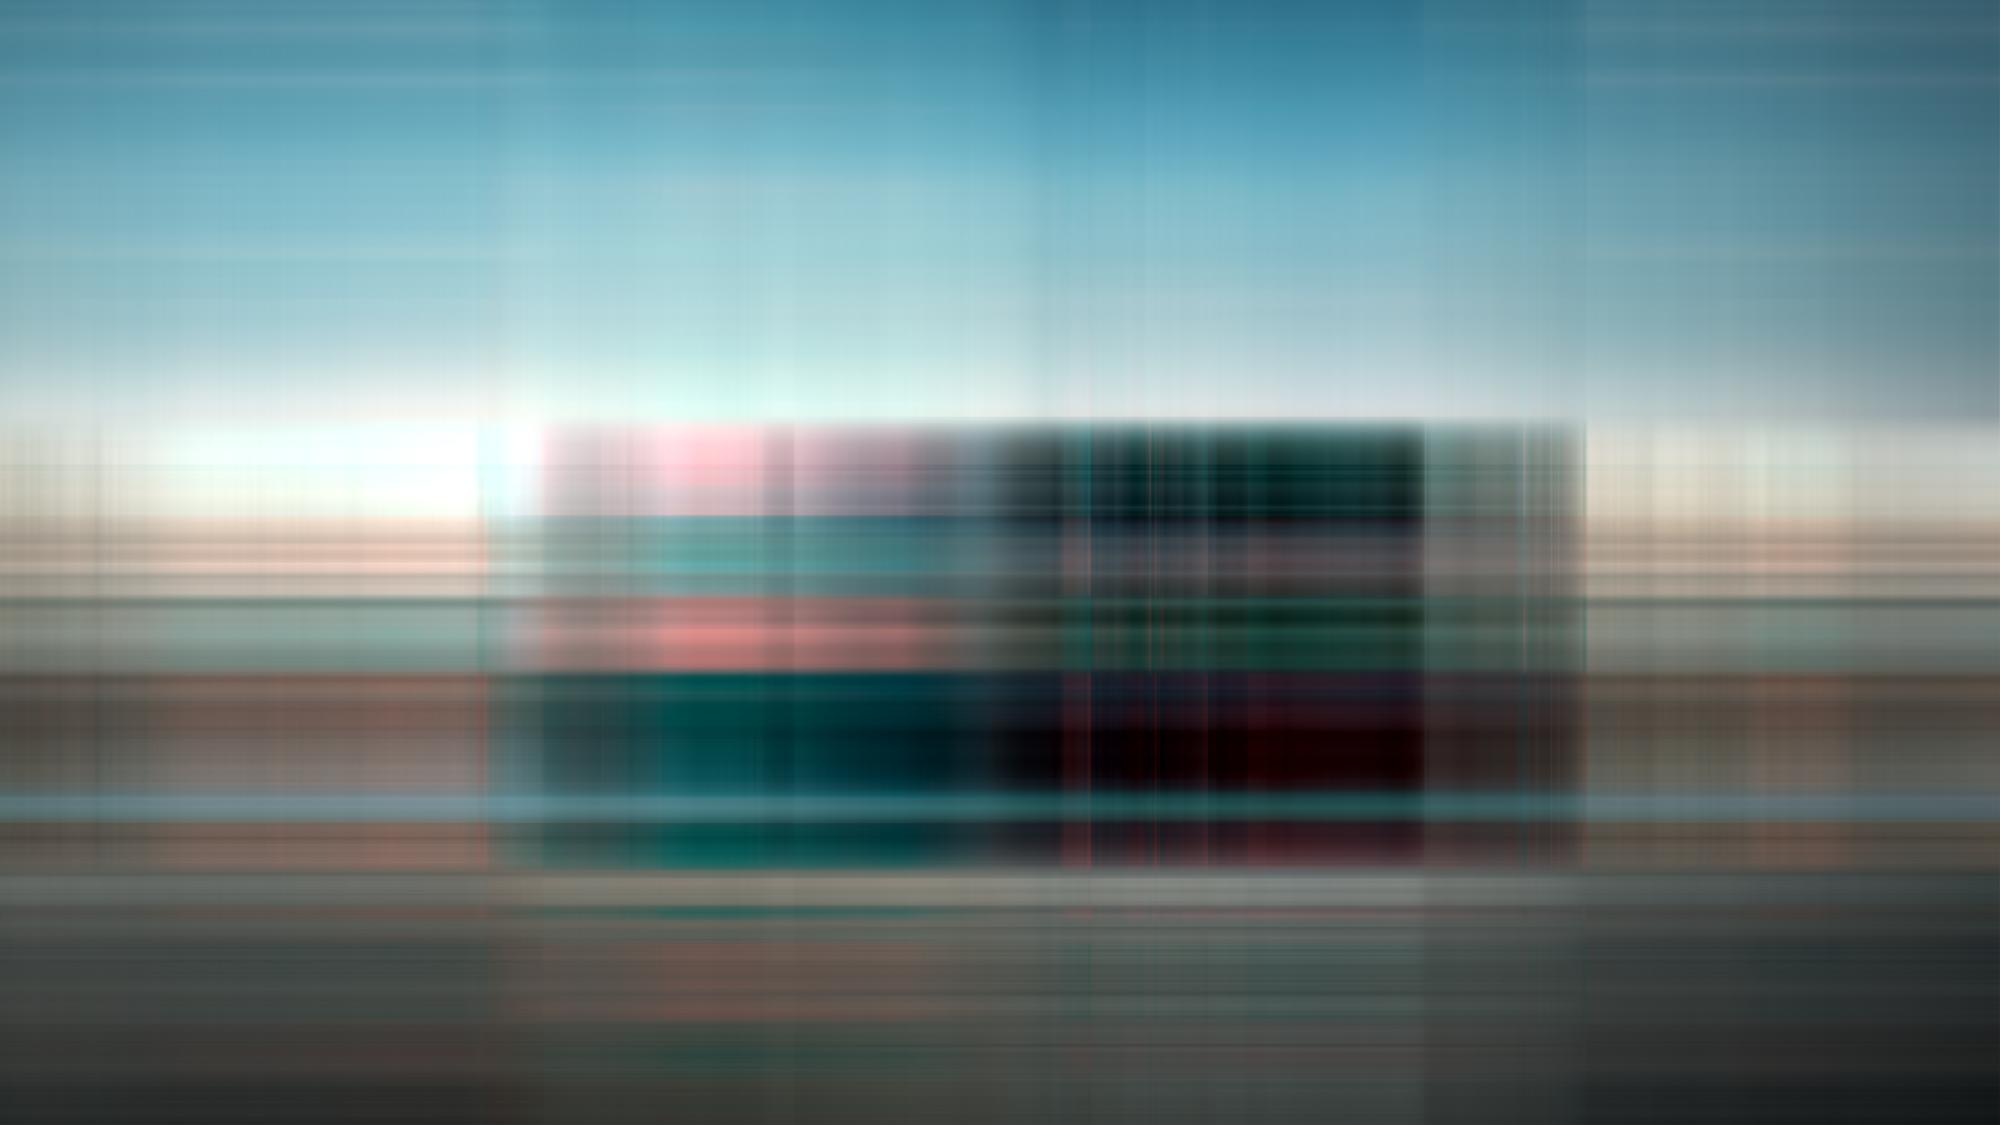
\includegraphics[width=5cm,height=3.5cm]{test3.jpeg}}		
		\centerline{保留30\%}	
	\end{minipage}
	\begin{minipage}{0.32\linewidth}	
		\vspace{3pt}
		\centerline{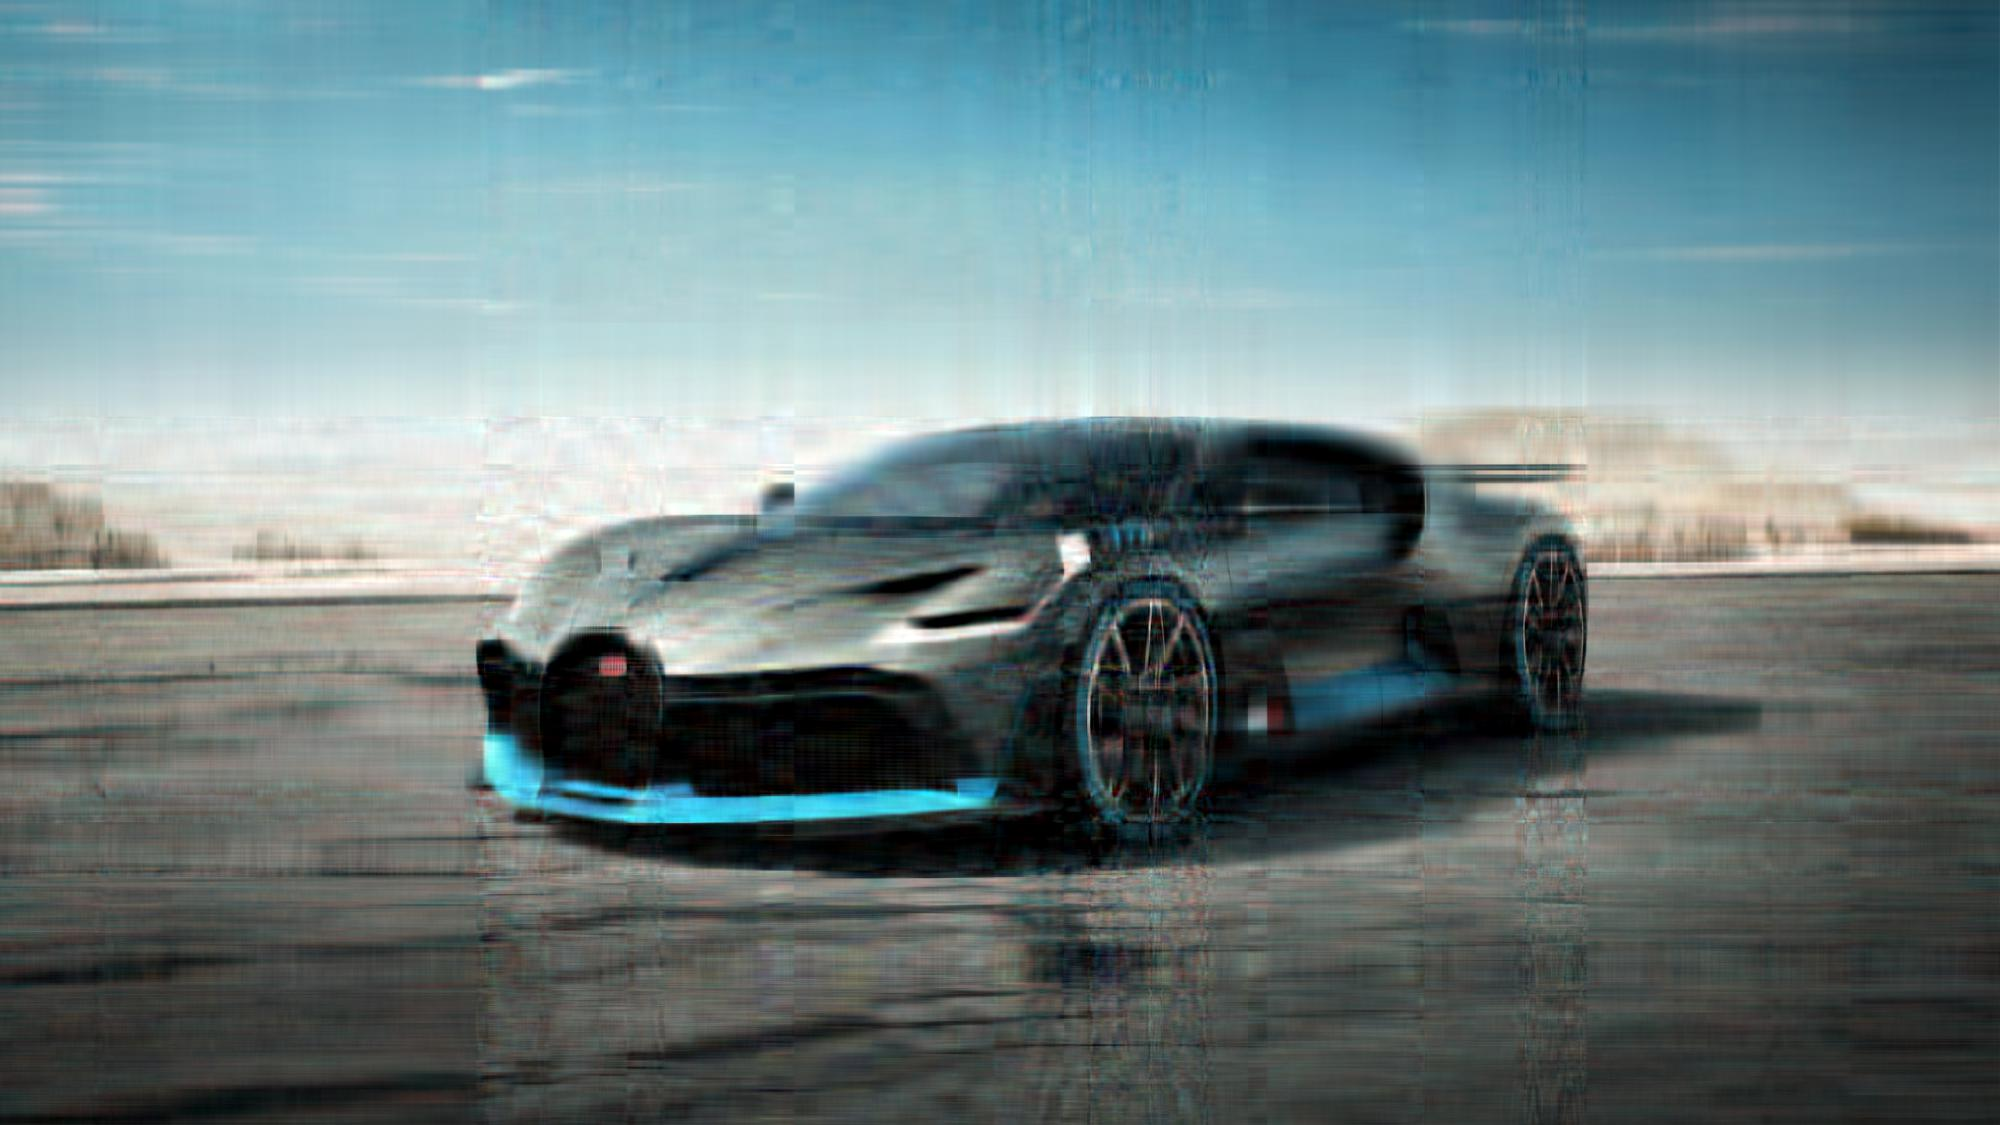
\includegraphics[width=5cm,height=3.5cm]{test5.jpeg}}
		\centerline{保留50\%}	
	\end{minipage}
	\begin{minipage}{0.32\linewidth}	
		\vspace{3pt}	
		\centerline{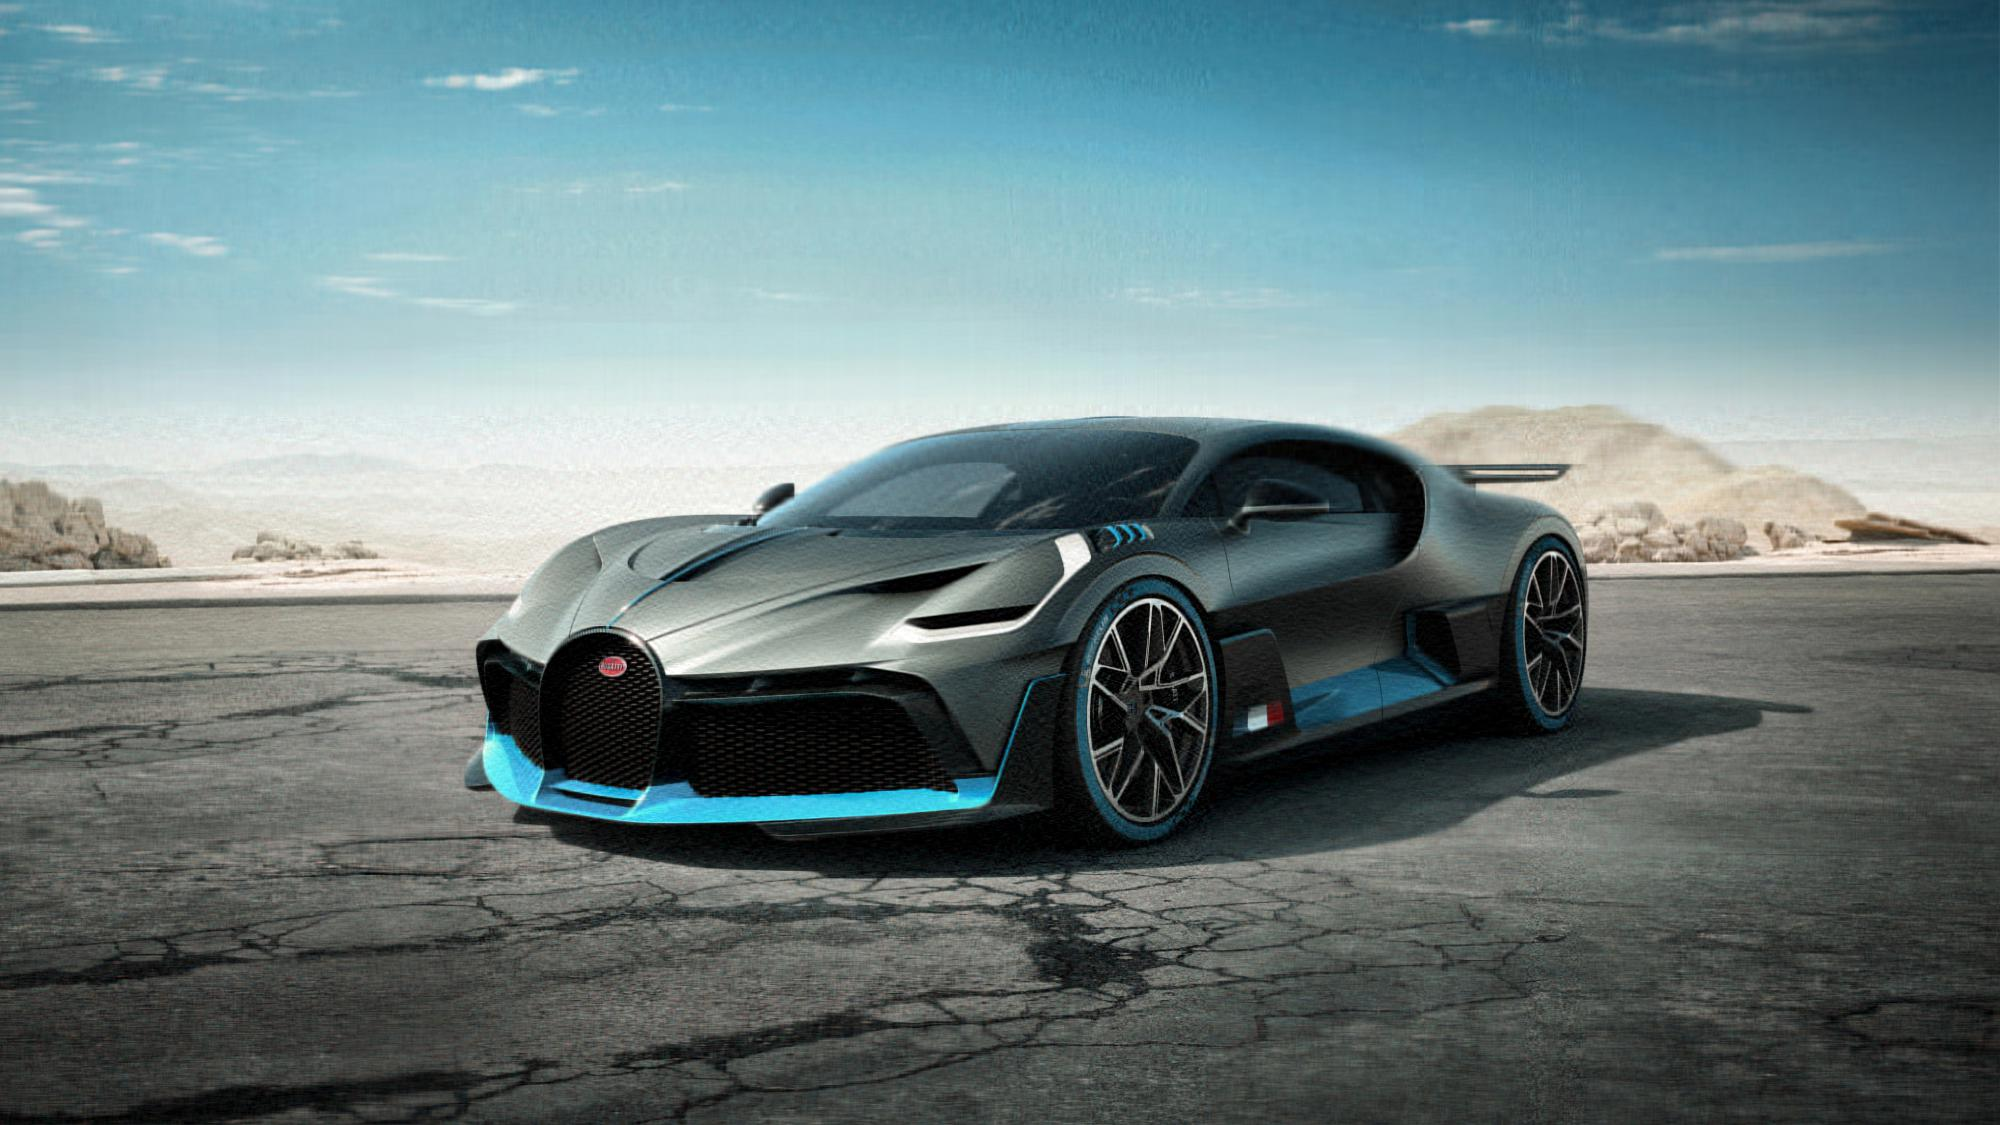
\includegraphics[width=5cm,height=3.5cm]{test7.jpeg}}	
		\centerline{保留70\%}	
	\end{minipage}
	\begin{minipage}{0.32\linewidth}	
		\vspace{3pt}	
		\centerline{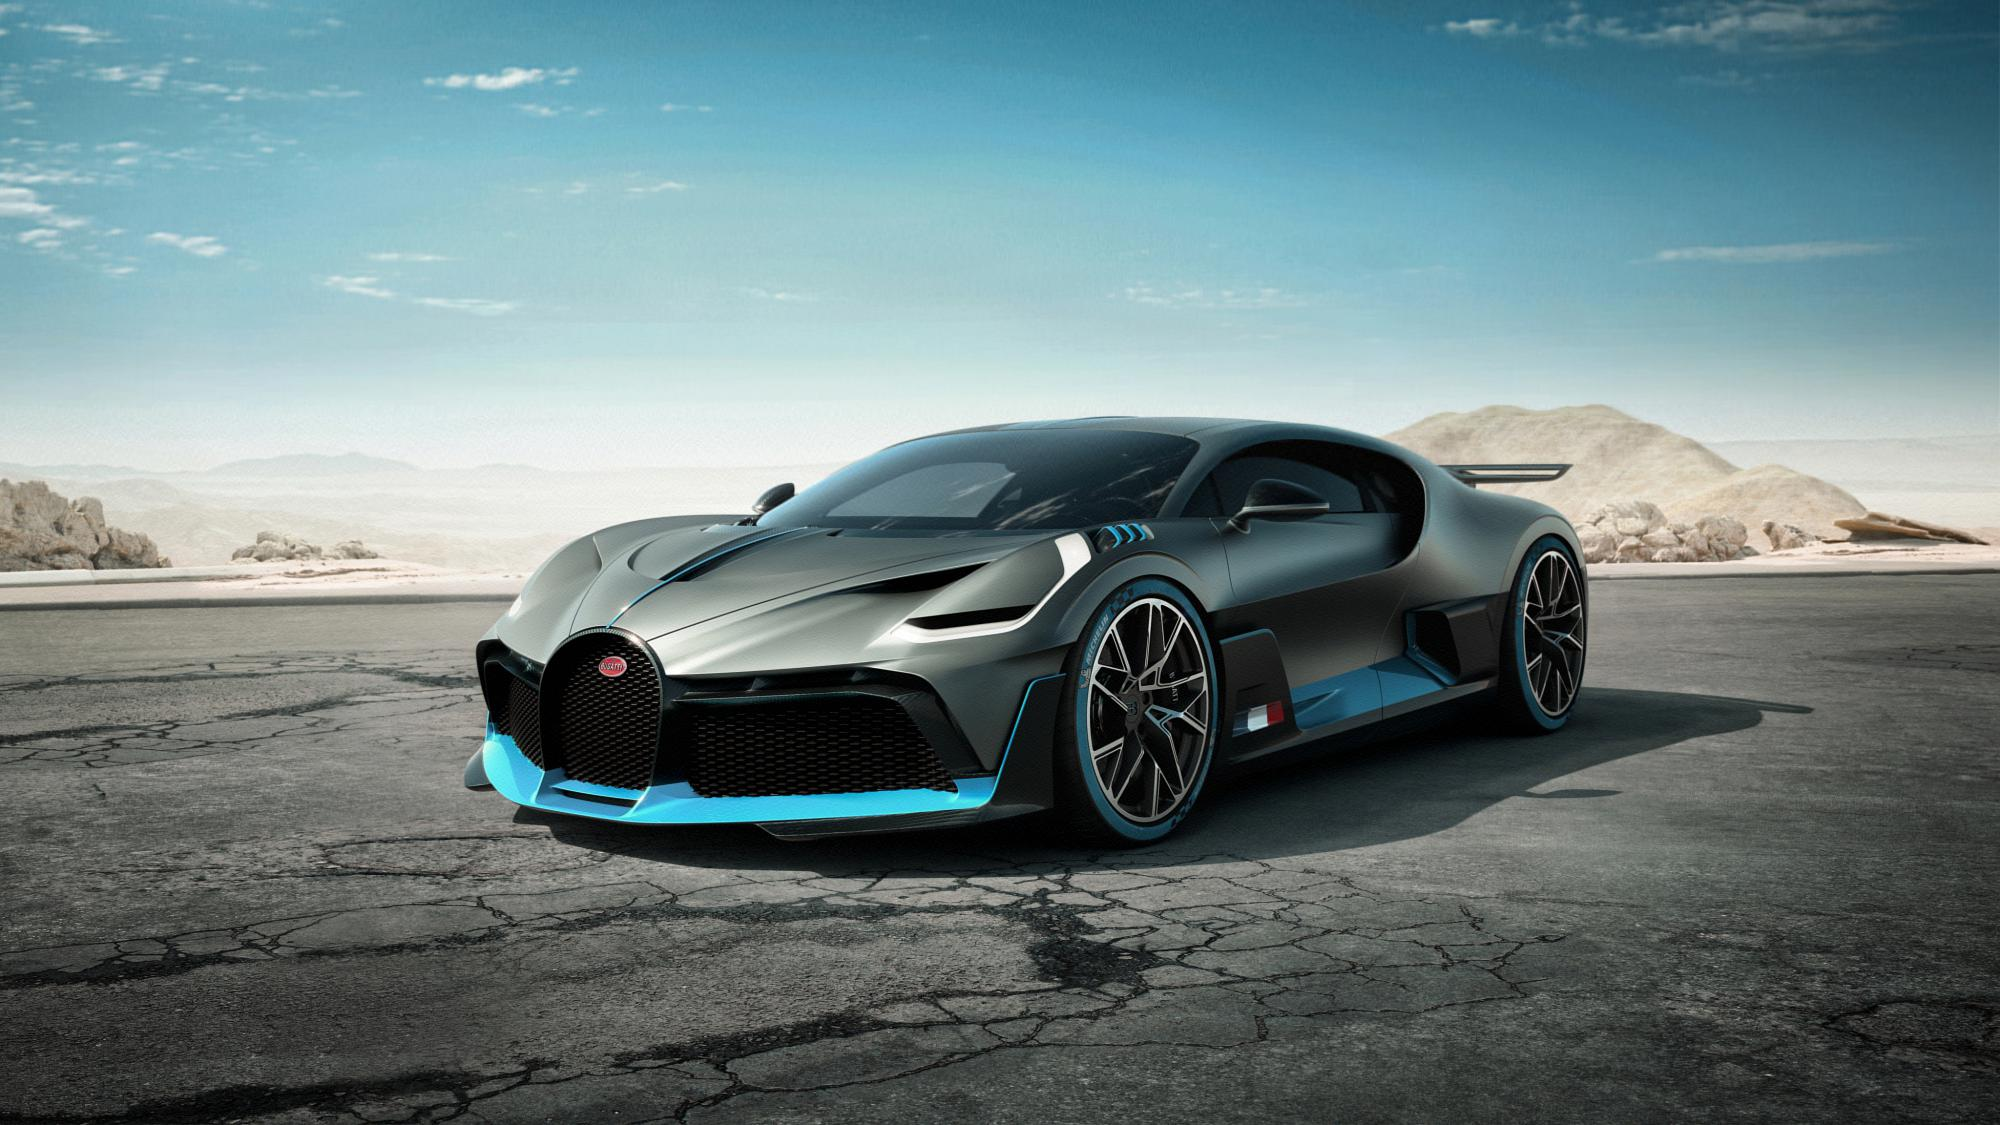
\includegraphics[width=5cm,height=3.5cm]{test9.jpeg}}		
		\centerline{保留90\%}	
	\end{minipage}
	\caption{原始图像与不同特征值保留比例压缩图像}
	\label{fig4}
\end{figure}
\subsubsection{主观评价方法}
人们对一幅图片视觉感受是主观评价,人自身对图像的评价是最为准确的。对于这种主观评价方法能参考国际电联ITU-R关于电视图像主观质量评价BT.500-13标准中的平均意见得分(MOS)方法(如图\ref{fig1}),就是通过人来观察图像,对图像的优劣进行主观评定(打分)。图像质量主观评价的MOS计分有两个尺度,即国际上通行的5级评分的质量尺度和损伤尺度。
\begin{figure}[H]
	\centering
	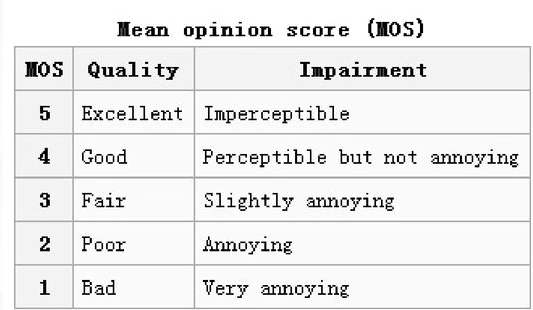
\includegraphics[scale=0.4]{MOS}
	\caption{图像主观质量的MOS分评价}
	\label{fig1}
\end{figure}

作者主观通过图\ref{fig4}原始图片与压缩完后的图片进行比较,不难发现对于原始图片压缩后只保留10\%,30\%和50\%的特征值直观上对于图片所要表达的信息有所缺失。相反的如果保留70\%和90\%的特征值的图片,依旧能够很好的表达图片的内容。主观的根据MOS分评价体系(图\ref{fig1})对上述不同特征值保留的图片进行打分如下表\ref{tab1}:
\begin{table}[h]
	\centering
	\begin{tabular}{|l|l|l|l|l|l|}
		\hline
		图片 & 保留10\%                 & 保留30\%                 & 保留50\%                 & 保留70\%                 & 保留90\%                 \\ \hline
		得分 & \multicolumn{1}{c|}{1} & \multicolumn{1}{c|}{2} & \multicolumn{1}{c|}{3} & \multicolumn{1}{c|}{4} & \multicolumn{1}{c|}{5} \\ \hline
	\end{tabular}
	\caption{图片主观打分}
	\label{tab1}
\end{table}

\subsubsection{客观评价方法}
由于本实验的实验目的是对于照片的压缩储存处理,故引入照片存储大小和尺寸两个对比因素。具体对比结果见下表\ref{tab2}。
\begin{table}[h]
	\centering
	\begin{tabular}{|c|c|c|c|c|c|c|}
		\hline
		图片 & 原图        & 保留90\%    & 保留70\%    & 保留50\%    & 保留30\%    & 保留10\%    \\ \hline
		尺寸 & 2000x1125 & 2000x1125 & 2000x1125 & 2000x1125 & 2000x1125 & 2000x1125 \\ \hline
		大小 & 1.4 MB    & 261.2 KB  & 230.7 KB  & 163.9 KB  & 91.9 KB   & 78.4 KB   \\ \hline
	\end{tabular}
	\caption{各基于特征值的压缩比例图片对比}
	\label{tab2}
\end{table}

本实验的压缩操作对于图片的尺寸没有进行压缩操作,而对于大小有较为明显的压缩。压缩完后图片大小与原始图片大小比例如下表\ref{tab3}。
\begin{table}[]
	\centering
	\begin{tabular}{|c|c|c|c|c|c|c|}
		\hline
		图片                         & 原图     & 保留90\%   & 保留70\%   & 保留50\%   & 保留30\%  & 保留10\%  \\ \hline
		大小                         & 1.4 MB & 261.2 KB & 230.7 KB & 163.9 KB & 91.9 KB & 78.4 KB \\ \hline
		\multicolumn{1}{|l|}{大小压缩比例} & 100\%  & 18.2\%   & 16.1\%   & 11.4\%   & 6.4\%   & 5.5\%   \\ \hline
	\end{tabular}
	\caption{各基于特征值的压缩比例大小压缩百分比}
	\label{tab3}
\end{table}

\section{结论}
综上所述,对于需要储存的大数据图片,SVD压缩是降低图片数据量的有效方法,而且依旧能够识别出重要的图像细节。它可以像滤波器一样用于图像去噪\cite{kolev2021big}。通过维纳滤波处理,SVD压缩速度更快。因此,与全秩图像相比,压缩图像在数据库中需要更少的计算机存储和传输时间,具有很大的应用场景。

\clearpage

\bibliography{demo}
\bibliographystyle{IEEEtran}

\clearpage

\section{对老师评价}

时光飞逝,不知不觉和邹老师度过了两个月的学习时间,在和老师学习的过程中受益匪浅。我能从老师身上学到许多课程之外的知识,教学方式有特色,教学具有启发式,为后续课程学习与实践训练打下很好的基础。老师幽默风趣,上课气氛活跃。老师和学生的互动性得到了充分的体现。我们从他那里学到的不仅仅是科学文化知识,更有学习方法和做人的道理。至于不好的方面,基本上没有,如果要挑的话,那就是在PPT制作过程中存在少数错误,偶尔会在课堂上扯到国际形势。
\end{document}